\chapter{Theoretical Study}
\label{cha:theoretical-study}

This chapter will explain in detail the taxonomy of \acrlong{fs} and delve into the concept of dimensionality reduction. It will also focus into the different \acrshort{fs} methods that exist and will end by explaining the concepts of complexity and stability, different metrics to apply to the results of the \acrshort{fs}.

\section{Taxonomy of FS}
\label{sec:taxonomy-fs}

\acrlong{fs} has many possibilities. \acrshort{fs} techniques do not alter the original representation of the variables, but merely select a subset of them (dimensionality reduction). Thus, they preserve the original semantics of the variables, hence, offering the advantage of interpretability by a domain expert \cite{Saeys2007}.

Unsupervised machine learning (clustering) and supervised machine learning (classification) are two main types of \acrshort{fs} techniques.

\textbf{Unsupervised learning} \cite{unsupervised-learning} uses unlabeled data to discover patterns that help solve grouping or association problems. This is particularly useful when those skilled in the art are unsure of common properties within a dataset.

\textbf{Supervised learning} \cite{supervised-learning} algorithms use labeled data to predict future outcomes or assign data to specific categories based on the regression or classification problem they are trying to solve. Although supervised learning algorithms tend to be more accurate than unsupervised learning models, they do require some initial human intervention to properly label the data. However, these labeled datasets allow supervised learning algorithms to avoid computational complexity, since they do not need a large training set to produce the expected results.

\textbf{Semi-supervised learning} occurs when only a portion of the given input data has been labeled. Unsupervised and semi-supervised learning may be a more attractive alternative, as it can be time consuming and costly to rely on domain expertise to properly label data for supervised learning.

While \acrshort{fs} can be applied to both supervised and unsupervised learning, we focus on the problem of supervised learning.

The advantages of \acrshort{fs} techniques come at a certain price, as the search for a subset of relevant features introduces an additional layer of complexity in the modelling task. \acrshort{fs} techniques differ from each other in the way they incorporate this search in the added space of feature subsets in the model selection.

In the context of classification, \acrshort{fs} techniques can be organized into three categories, depending on how they combine the \acrlong{fs} search with the construction of the classification model: filter methods, wrapper methods and embedded methods.

In the \textbf{Filter method}, features are selected based on statistical measures. In most cases a feature relevance score is calculated, and low-scoring features are removed. Advantages of filter techniques are that they easily scale to very high-dimensional datasets, they are computationally simple and fast, and they are independent of the classification algorithm. Some disadvantages of the filter method are that it ignores feature dependencies, and the advantage of being classifier-independent becomes a disadvantage of ignoring interaction with it. Binary consistency, chi-square, cramer, r squared, gini index, \acrlong{mdlc}, mutual information, relief are some of the statistical measures used to understand the importance of the features. See an example of using determination coefficient filter method measure in Section \ref{sec:measures-fsinr}.

The \textbf{Wrapper methodology} considers the selection of feature sets as a search problem, where different combinations are prepared, evaluated and compared with other combinations. A predictive model \footnote{Predictive Models are a set of techniques that aim to provide a prediction of future results in order to specify decision-making through data analysis techniques.} is used to evaluate a combination of features and assign model performance scores. Advantages of wraparound approaches include the interaction between feature subset search and model selection, and the ability to account for feature dependencies. A common drawback of these techniques is that they have a higher risk of overfitting than filter techniques and are computationally intensive, especially if building the classifier has a high computational cost. Some examples of this method are Sequential forward selection, Sequential backward elimination, Backward variable selection (see Section \ref{sec:valselrf-package}) or \acrfull{rfe} (ee Section \ref{sec:caret-package}).

In \textbf{Embedded techniques}, the feature selection algorithm is integrated as part of the learning algorithm. Like enveloping approaches, embedded approaches are specific to a given learning algorithm. Embedded methods have the advantage that they include interaction with the classification model and, at the same time, are much less computationally intensive than wraparound methods. In the same way, the dependency of the selection on the classifier can be a disadvantage in some cases. The most typical integrated technique is the decision tree algorithm. Decision tree algorithms select a feature at each recursive step of the tree growth process and divide the set of samples into smaller subsets.

Focusing now on the filter methods, these are divided into univariate or multivariate.

Most of the proposed techniques are \textbf{univariate}. This means that each variable is considered separately, thus ignoring the dependencies of different variables, which can lead to poorer classification performance compared to other types of \acrshort{fs} techniques. This leads to a common disadvantage of filter methods.

To overcome the problem of ignoring feature dependencies, a number of \textbf{multivariate} filter techniques were introduced, with the goal of incorporating feature dependencies to some extent. The term multivariate technique refers to the fact that more than one variable is used in its metrics.

If the univariate technique is applied, simple metrics will be used that are calculated with a single variable, such as the mean, the median or dispersion measures such as the range or standard deviation. On the other hand, a simple form of multivariate technique is to create a scatterplot matrix, which is a matrix that displays a scatterplot for each pairwise combination of numeric variables in the data set. With it you can visualize the relationship between two or more variables at the same time.

After introducing and explaining the different \acrshort{fs} techniques, Figure \ref{fig:techniques} shows a schematic summary of the previously seen types.

\begin{figure}[H]
    \centering
    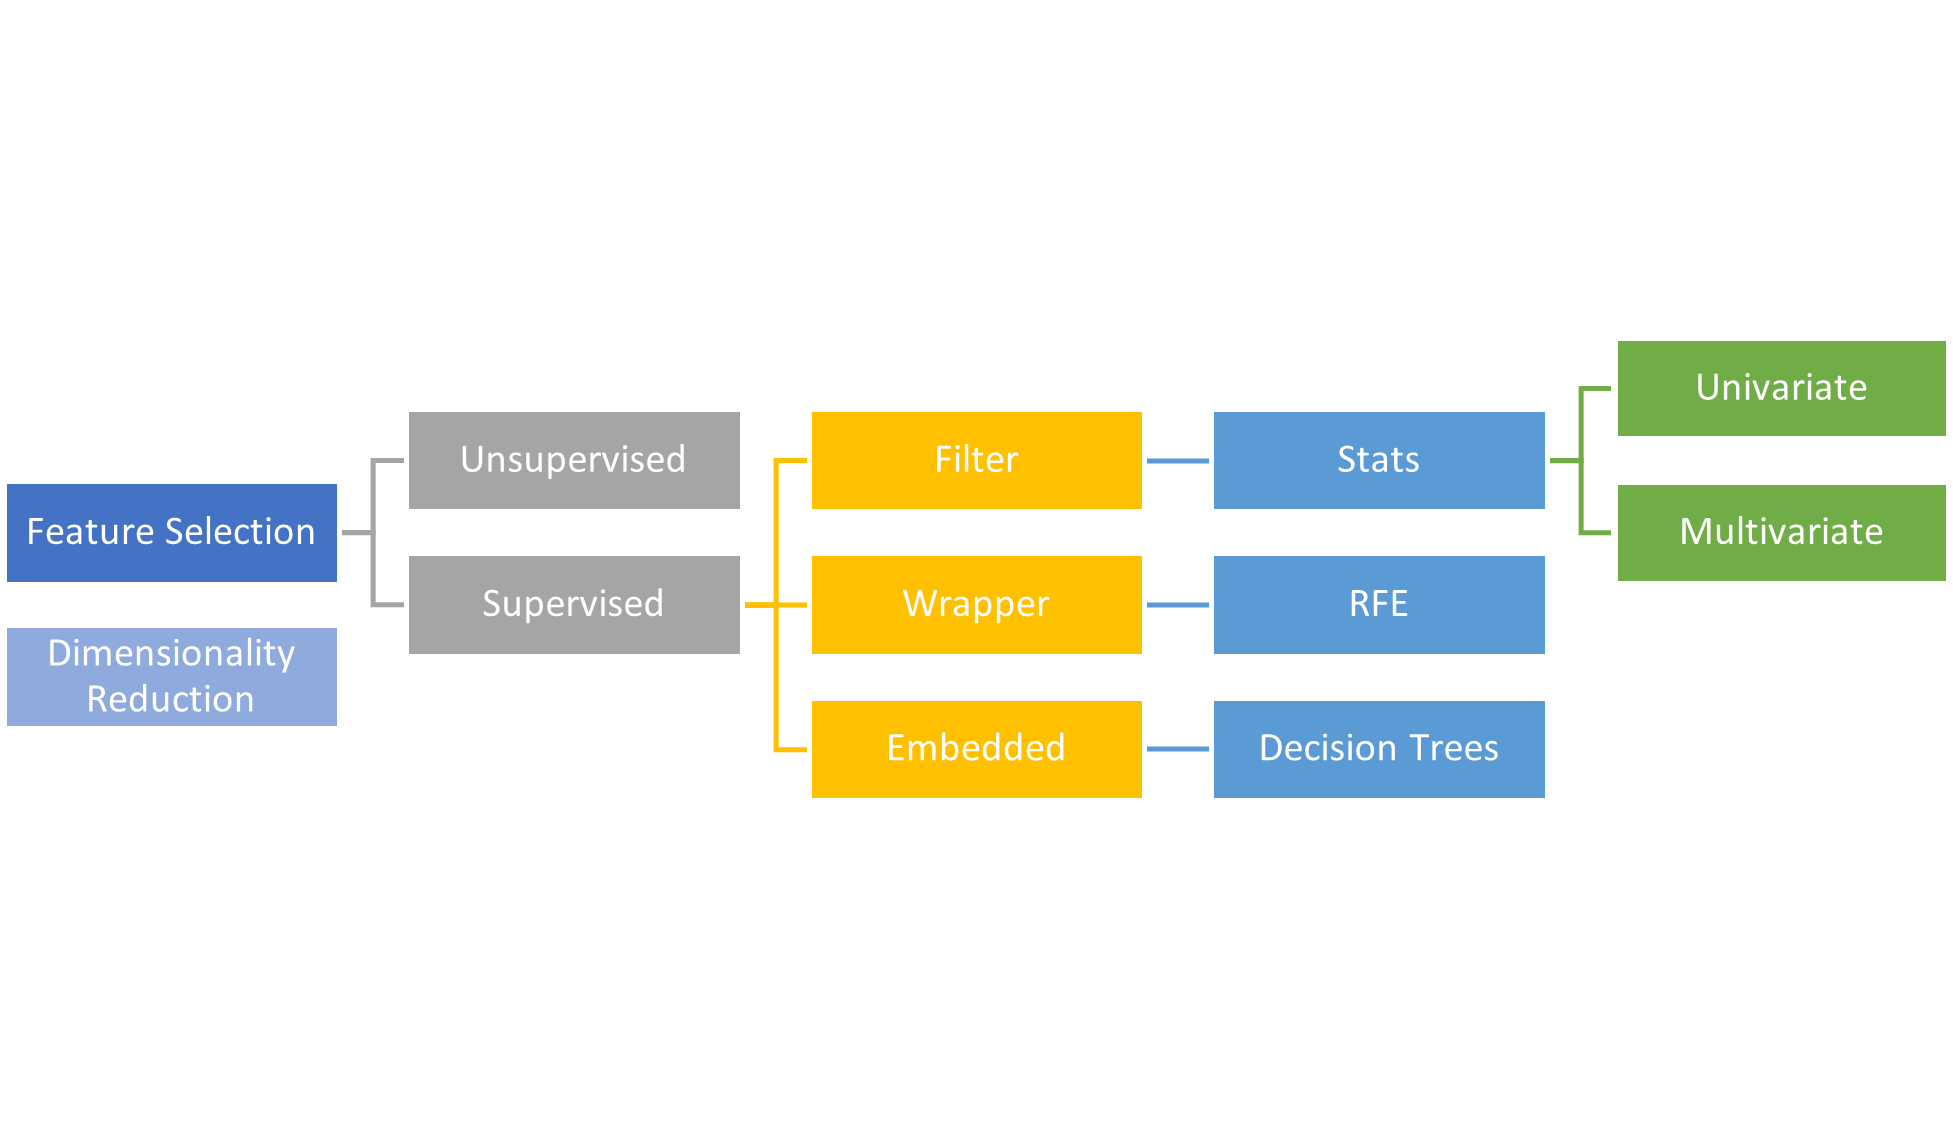
\includegraphics{techniques.png}
    \caption{\acrlong{fs} techniques \cite{fs-method-ml}.}
    \label{fig:techniques}
\end{figure}

\subsection{Dimensionality Reduction}
\label{sec:dimensionality-reduction-1}

Dimensionality of a dataset is the number of input variables or features of these dataset. With this it is concluded that techniques used to reduce the number of input variables are called dimensionality reduction \cite{dimensionality-reduction}. Reducing dimensionality produces a more compact representation in which it is easier to interpret the target variable, focusing attention on the most relevant variables, better understanding of the data, decreased time and storage in measurements and training, etc.

Dimensionality reduction transform the input data into a lower-dimensional feature space that retains meaningful properties of the original data.

The more input features there are in a dataset, the more difficult it is to create a predictive model for machine learning algorithms to study the data with. One of the main drawbacks is the computational cost involved in processing a large amount of data to carry out this predictive model.

If the data is represented by rows and columns, such as in a matrix, the features are the columns that are fed as input to a model to predict the target variable.

Dimensionality reduction techniques are commonly used in data visualization because it is not easy to see large dimensions of data. The goal of dimensional reduction for data visualization is to transform data until it can be represented in 2- or 3-dimensional form so that humans can understand its structure. People are generally interested in visualizing whether data has cluster structures or curves and doing so in a more intuitive way.

For example, features matrix can be considered where the columns of data represent dimensions in an n-dimensional feature space and the rows of data as points in that space. This is a useful geometric interpretation of a dataset. Having a large number of dimensions (many columns) in the feature space, the points that we have in that space (rows of data) often represent a small and non-representative sample.

Nevertheless these dimensionality reduction techniques can be used in applied machine learning in order to better fit a predictive model.

In linear models, the number of inputs and the degrees of freedom \footnote{Degrees of freedom are often defined as the number of observations (pieces of information) in the data that are free to vary when estimating statistical parameters.} of the model are often closely related. Most likely, a model with too many degrees of freedom will fit the training data set too well and therefore not perform well with the new data. The ideal is to have simple models that generalize well and, at the same time, have input data with few input variables.

There are two ways to reduce of the dimensionality of classification problems and should be distinguished from each other: 

\begin{itemize}
    \item \textbf{\acrfull{fss}} \cite{GuyonElisseeff2003} consists of selecting the best subset of features for the classification purpose.

    \item \textbf{Feature extraction} \cite{liu1998feature} consists of combining the features in the dataset to obtain new better features. These new features are created from functions of the original features. In this approach, the meaning of the original variables is lost in the newly constructed features.
\end{itemize}

It is common to use the two techniques in combination, but in this case the focus will be on \acrlong{fss} and the selection of the most important attributes.

\section{Feature Subset Selection}
\label{sec:fss}

\acrlong{fs} is also known as variable selection, attribute selection, variable subset selection or \textbf{\acrfull{fss}}.

As already mentioned in Section \ref{sec:preprocessing}, \acrshort{fss} is an important part of the preprocessing step in \acrfull{kdd} (Section \ref{sec:kdd-process}). Using \acrshort{fss} algorithms has important benefits for data mining:
\begin{itemize}
    \item A reduced volume of data allows different data mining or searching techniques to be applied. Some techniques would be unfeasible if the dataset is very large due to the lack of resources to process it correctly and obtain an optimal result.

    \item Irrelevant and redundant attributes can generate less accurate and more complex models. These types of attributes are not necessary as they only prevent efficient execution of the learning algorithms. Furthermore, data mining algorithms can be executed faster the smaller the input dataset.

    \item We can avoid the collection of data for those irrelevant and  redundant attributes in the future. This is positive for the processing part since the information that this type of attribute can offer is not necessary and would be equally irrelevant and redundant.
\end{itemize}

\acrshort{fss} algorithms search through candidate feature subsets guide by a certain evaluation measure which captures the goodness of each subset. It is intended to select the subset of features that contributes most significantly to machine learning.

To propose a general example, we imagine a data set with 5 features: blood pressure, weight, height, blood glucose and diabetes. The goal is to predict whether future patients will develop diabetes from data collected from current patients. With the \acrshort{fss} algorithms, it can be concluded that height has no effect on the development of diabetes and, therefore, this characteristic can be ruled out. This reduces the size of the dataset to 4 features. With this new data subset, it is intended to improve the results than using the full dataset.

An optimal (or near optimal) subset is selected when the search stops. This means that the algorithm has already examined all possible combinations of features to find the feature sets that best satisfy the predetermined criteria \cite{optimal}.

As already presented in Section \ref{sec:taxonomy-fs} above, \acrlong{fs} methods generally come in three classes depending on how they combine the selection algorithm and model building: filter methods, wrapper methods and embedded methods. The first two are the ones that will be discussed in the Experimental Work (Chapter \ref{cha:experimental-work}), so they will be broken down in the following sections.

\section{Complexity}
\label{sec:complexity}

Complexity is used to measure the behavior of a system or model. Its components interact in multiple ways, which means that their behavior is random and not linear. Therefore, it can be stated that it is possible to measure the complexity of classification problems such as \acrlong{fs}.

The error rate is a very useful measure to know the difficulty of a problem, but sometimes more independent measures are needed to obtain more information about the complexity of a dataset. In other words, using a single measure may not be enough and you may have to consider using a number of different measures \cite{TinKamHoBasu2002}.

There are a set of measures that help characterize the complexity of classification and regression problems. The measurements are as follows:

\begin{itemize}
    \item \textbf{Overlapping:} Evaluate how informative the features available to separate the classes are.
    
    \item \textbf{Neighborhood:} Characterize the presence and density of classes in local neighborhoods.
    
    \item \textbf{Linearity:} Quantify, if possible, whether the classes are linear separable by a hyperplane or a linear function.
    
    \item \textbf{Dimensionality:} Indicative of data sparseness, how well samples are distributed within attributes. The degree of high dimensionality that datasets have.
    
    \item \textbf{Balance:} Capture the difference in the number of examples per class in the dataset.
    
    \item \textbf{Network:} Represents the dataset as a graph and extracts structural information from it.
    
    \item \textbf{Correlation:} Relationship between the feature values and the outputs.
    
    \item \textbf{Smoothness:} In regression problems, the smoother the function is in fitting the data, the simpler it is.
\end{itemize}

These complexity measures will be calculated for a particular dataset, before and after feature selection, and comparisons will be made between the results. See Section \ref{sec:ecol-package}.

\section{Stability}
\label{sec:stability}

Stability means the insensitivity of the result of a \acrlong{fs} algorithm to variations in the training dataset. A feature selection algorithm with no stability constraint typically results in significantly different feature subsets due to variations in the training data \cite{LiSiZhou2015}.

If different datasets but with the same features are applied to a feature selection algorithm, the algorithm has to return the same features as important in all of them.

Stability measurement is important as it addresses a fundamental question in data science: trust in algorithms. If small changes in the initial conditions result in significantly different conclusions, perhaps we should not trust the output it reflects.

The stability value obtained is an estimate of a true stability since it depends on the number of feature sets sampled. Starting from this statement, Nogueira, Sechidis and Brown provide an estimator and a theoretical analysis of its properties in the paper "On the Stability of Feature Selection Algorithms" \cite{JMLR2018}.

In Section \ref{sec:stability-fsinr} an example of the use of the stability measure proposed in the mentioned paper will be made.

\section{SHAP Values}
\label{sec:shap-values}

Given a predictive model and a predicted case, it is interesting to know the impact of each predictor variable in the model on the prediction.

The value of the impact of each variable is known as the SHAP value, in honor of the american mathematician and economist Lloyd Shapley. His idea was to distribute in a fair way among the players the benefit obtained by a team, taking into account how much the presence of each player contributed to each 'sub-team'. The players would become the predictor variables. Each 'sub-team', a subset of variables \cite{shap}.

In additive models, for example, $f(x_1, x_2) = 2x_1 -3x_2 + 4$, the contribution of the value of each variable in the prediction made by f is the same for all instances since the variables do not interact with each other. The coefficient of the variables in the model indicates the magnitude of the contribution. There are variables that do interact in other models and the contribution-impact of the value of a variable in the prediction depends on the values of the rest of the variables.

If the number of variables grows, it is not computationally possible to perform all the calculations. Therefore, to approximate the real value of the SHAP value, a random sampling of subsets of variables is performed. An amount is fixed, based on the computational resources available. There are several methodologies for calculating SHAP values. In libraries you will find different implementations for different types of classifiers. In Section \ref{sec:shap-package} you will see an example of calculating the SHAP values.